
%(BEGIN_QUESTION)
% Copyright 2015, Tony R. Kuphaldt, released under the Creative Commons Attribution License (v 1.0)
% This means you may do almost anything with this work of mine, so long as you give me proper credit

\noindent
{\bf Lab Exercise -- introduction}

\vskip 5pt

Your task is to modify the PID-controlled process constructed in the previous lab exercise to include monitoring and/or control using one or more FOUNDATION Fieldbus instruments, then document and troubleshoot the complete system.

The following table of objectives show what you and your team must complete within the scheduled time for this lab exercise.  Note how some of these objectives are individual, while others are for the team as a whole:

\underbar{Objective completion table:}

% No blank lines allowed between lines of an \halign structure!
% I use comments (%) instead, so that TeX doesn't choke.

$$\vbox{\offinterlineskip
\halign{\strut
\vrule \quad\hfil # \ \hfil & 
\vrule \quad\hfil # \ \hfil & 
\vrule \quad\hfil # \ \hfil & 
\vrule \quad\hfil # \ \hfil & 
\vrule \quad\hfil # \ \hfil & 
\vrule \quad\hfil # \ \hfil & 
\vrule \quad\hfil # \ \hfil \vrule \cr
\noalign{\hrule}
%
% First row
{\bf Performance objective} & {\bf Grading} & {\bf 1} & {\bf 2} & {\bf 3} & {\bf 4} & {\bf Team} \cr
%
\noalign{\hrule}
%
% Another row
Circuit design challenge & mastery & & & & & -- -- -- -- \cr
%
\noalign{\hrule}
%
% Another row
Fieldbus segment diagram and inspection & mastery & & & & & -- -- -- -- \cr
%
\noalign{\hrule}
%
% Another row
Demonstration of working Fieldbus instrument & mastery & -- & -- & -- & -- & \cr
%
\noalign{\hrule}
%
% Another row
Troubleshooting & mastery & & & & & -- -- -- -- \cr
%
\noalign{\hrule}
%
% Another row
Lab question: Instrument connections & proportional &  &  &  &  & -- -- -- -- \cr
%
\noalign{\hrule}
%
% Another row
Lab question: Commissioning & proportional &  &  &  &  & -- -- -- -- \cr
%
\noalign{\hrule}
%
% Another row
Lab question: Mental math & proportional &  &  &  &  & -- -- -- -- \cr
%
\noalign{\hrule}
%
% Another row
Lab question: Diagnostics & proportional &  &  &  &  & -- -- -- -- \cr
%
\noalign{\hrule}
%
% Another row
Lab clean-up & mastery & -- & -- & -- & -- &  \cr
%
\noalign{\hrule}
} % End of \halign 
}$$ % End of \vbox

The only ``proportional'' scoring in this activity are the lab questions, which are answered by each student individually.  A listing of potential lab questions are shown at the end of this worksheet question.  The lab questions are intended to guide your labwork as much as they are intended to measure your comprehension, and as such the instructor may ask these questions of your team day by day, rather than all at once (on a single day).

\vskip 10pt

{\bf It is essential that your team plans ahead what to accomplish each day.  A short (10 minute) team meeting at the beginning of each lab session is a good way to do this, reviewing what's already been done, what's left to do, and what assessments you should be ready for.  There is a lot of work involved with building, documenting, and troubleshooting these working instrument systems!}

As you and your team work on this system, you will invariably encounter problems.  You should always attempt to solve these problems as a team before requesting instructor assistance.  If you still require instructor assistance, write your team's color on the lab whiteboard with a brief description of what you need help on.  The instructor will meet with each team in order they appear on the whiteboard to address these problems.





\vfil \eject

\noindent
{\bf Lab Exercise -- circuit design challenge}

\vskip 5pt

Connect a loop-powered ``smart'' differential pressure transmitter (4-20 mA output with HART communication ability) to a DC voltage source and a meter such that the meter will indicate a increasing signal when a certain stimulus is applied to the transmitter, setting the transmitter's pressure measurement range as specified by the instructor.  All electrical connections must be made using a terminal strip (no twisted wires, crimp splices, wire nuts, spring clips, or ``alligator'' clips permitted).  You are expected to supply your own tools and multimeter.

This exercise tests your ability to navigate a ``smart'' instrument's parameters using a communicator as well as properly interpret terminal connections on a field instrument for signal and power.

$$\includegraphics[width=15.5cm]{i03600x01.eps}$$

\vskip 10pt

The following components and materials will be available to you: assorted 2-wire 4-20 mA differential pressure {\bf transmitters} calibrated to ranges 0-30 PSI or less, equipped with Swagelok compression tube connectors at the ``high'' and ``low'' ports ; lengths of {\bf plastic tube} with ferrules pre-swaged ; {\bf terminal strips} ; lengths of {\bf hook-up wire} ; 250 $\Omega$ (or approximate) {\bf resistors} ; analog {\bf meters} ; {\bf battery clips} (holders); {\bf HART communicator}.

\vskip 10pt

\noindent
{\bf Transmitter range} (instructor chooses): \hskip 20pt LRV = \underbar{\hskip 50pt} \hskip 20pt URV = \underbar{\hskip 50pt}

\vskip 10pt

\noindent
{\bf Meter options} (instructor chooses): \hskip 20pt \underbar{\hskip 20pt} Voltmeter (1-5 VDC) \hskip 10pt {\it or} \hskip 10pt \underbar{\hskip 20pt} Ammeter (4-20 mA)

\vskip 10pt

\noindent
{\bf Signal increases with...} (instructor chooses): \hskip 20pt \underbar{\hskip 20pt} Positive pressure \hskip 10pt {\it or} \hskip 10pt \underbar{\hskip 20pt} Vacuum (suction)

\vskip 10pt

\vfil

Study reference: the ``Analog Electronic Instrumentation'' chapter of {\it Lessons In Industrial Instrumentation}, particularly the sections on loop-powered transmitters and current loop troubleshooting.  Also, the ``Basic Concept of HART'' subsection of the ``The HART Digital/Analog Hybrid Standard'' section of the ``Digital Data Acquisition and Networks'' chapter of the same book.





\vfil \eject

\noindent
{\bf Lab Exercise -- commissioning a new Fieldbus instrument}

\vskip 5pt

The Instrumentation lab is set up to host FOUNDATION Fieldbus instruments via several couplers located at central points in the ``rack'' system.  Simply take a Fieldbus instrument, wire a quick-disconnect connector to it, and plug it into any one of these couplers to install it on an H1 segment.  The two couplers on the north end of the lab are on their own H1 segment (connected to Port 2 on the north DeltaV DCS rack H1 card), while the two couplers on the south end of the lab are on their own H1 segment as well (connected to Port 1 on the north DeltaV DCS rack H1 card).  At this point in time the south DeltaV DCS rack has no H1 interface card.

Your first step should be selecting a proper FOUNDATION Fieldbus instrument to make part of your working system.  If your choice of measurement variable is temperature, it is recommended that you partner with another team using temperature as well so that you may make double-use of a Fieldbus multi-channel temperature transmitter (Rosemount 848T).

The next step should be finding appropriate documentation for your Fieldbus transmitter.  Nearly every instrument in the lab is documented electronically at the manufacturer's website, so your best resource is the Internet (and/or your Instrumentation Reference where a variety of instrument manuals have been downloaded for you).  Use this documentation to identify how to properly wire, power, and calibrate the transmitter.  Your instructor will insist upon a simple sketch of your planned wiring before connecting your Fieldbus transmitter to the H1 segment.

Finally, you will need to commission the Fieldbus transmitter so that it is recognized by the DCS host.  Refer to your {\it Lessons In Industrial Instrumentation} textbook and to your DCS documentation for details on how to do this.  Once commissioned, your team's Fieldbus instrument will appear in the ``tree'' style directory in the DeltaV Explorer window, and its overall status will register as ``Good.''  

A very important point to remember when working with the DeltaV system is that all changes must be downloaded (all blue triangle symbols must be eliminated) at the conclusion of each commissioning action and after each decommissioning action.  If any changes are made without downloading, the DeltaV system will be in an uncertain state, causing problems for the next team trying to commission or decommission their Fieldbus instrument!  {\it For this reason, it is highly advisable for teams to take turns when commissioning/decommissioning their Fieldbus instruments (i.e. only one team at a time per DeltaV node) in order to avoid making new changes before the last change gets downloaded.}

\vskip 10pt

{\bf Common mistakes:}

\begin{itemize}
\item{} Neglecting to consult the manufacturer's documentation for field instruments (e.g. how to wire them, how to calibrate them).
\item{} Not carefully examining the Fieldbus plug (quick-disconnect) pinout, and getting the wiring wrong where the instrument plugs in to the coupling device.
\item{} Students working on portions of the system in isolation, not sharing with their teammates what they did and how.  It is important that the whole team learns all aspects of their system!
\end{itemize}

\vskip 10pt

{\bf Commissioning a new Fieldbus instrument should take no more than an hour for a team doing it for the very first time, assuming they follow the instructions shown in the textbook.}






\vfil \eject

\noindent
{\bf Lab Exercise -- configuring function blocks for a new Fieldbus instrument}

\vskip 5pt

After commissioning your team's Fieldbus transmitter, you must create a function block program to use the data available in that transmitter.  Some function block ``Modules'' have already been created in the DeltaV system (associated with the north DCS node, ``CTRL-1'') to hold the Fieldbus function blocks.  Note that you should not try to mix Fieldbus instruments on different segments (i.e. different ports on the H1 card) within the same module (the same function block diagram).  Rather, communications between Fieldbus instruments should occur within the same H1 network segment.

Using Control Studio to edit the module, paste an ``Analog Input'' function block on the screen and assign that block to the Fieldbus instrument of your choice.  Your next step should be to set the target operating mode of this new function block to ``OOS'' (Out Of Service).  While technically unnecessary at this point (since your new AI block doesn't connect to any other function blocks yet and therefore cannot affect anything else), this is a good habit to get into because it prevents any configuration-related changes in that block from affecting any ``downstream'' function blocks in a real system.

After setting the mode to OOS, set the {\tt Channel} parameter within the AI function block to access the desired data channel within the Fieldbus instrument.  If your instrument is a Rosemount 848T temperature transmitter, for example, channels 1 through 8 signify the eight different temperature signal inputs on this multi-input transmitter.  If your instrument is a Rosemount model 3095 DP transmitter, the different channels (1 through 5) represent differential pressure, static pressure, process temperature, internal temperature, and calculated mass flow, respectively.  Consult the manual for your Fieldbus instrument to obtain more detail on channels.

Then, set the {\tt L\_type}, {\tt XD\_Scale}, and {\tt OUT\_Scale} parameters of the Analog Input block to properly range the block's output signal.  For example, if you were ranging a pressure instrument to function as a liquid level instrument, this is where you would set the pressure ({\tt XD\_Scale}) and level ({\tt OUT\_Scale}) high and low ranges, so that a specified range of sensed pressures would translate into a specified range of liquid levels (or liquid mass, or liquid volume, depending on how you wished to represent the liquid quantity to the operator).  You will find details on these parameters within the manual for your instrument as well as within your {\it Lessons In Industrial Instrumentation} textbook.

After configuring these AI block parameters, return the function block to its ``Auto'' mode so that the output will now respond to the live instrument.  When completed, you should have an Analog Input function block outputting a scaled measurement in some real-world unit (e.g. PSI, degrees Fahrenheit, etc.), ready to be connected to a PID or other function block in that module.  You may monitor the value of your AI block's signal using the ``Online'' or ``Debug'' modes of Control Studio, or alternatively you may configure DeltaV Operate to display and graph the instrument's signal where any operator can see it.

\vskip 10pt

An interesting exercise you may do after configuring the AI function block is to put that block into ``manual'' mode (set the target value to Manual), where you may force the output of that function block to whatever value you desire.  This is a useful tool for testing and troubleshooting function block programs, and it is a feature supported by every Fieldbus function block.  Be sure to switch the block's target mode back to Auto when you are finished!

\vskip 10pt

{\bf Common mistakes:}

\begin{itemize}
\item{} Not properly setting the {\tt Channel} parameter in the AI block, and thus acquiring the wrong data from the instrument. 
\item{} Leaving the {\tt L\_type} parameter set to ``Direct'' when you wish to scale the signal.
\item{} Failing to set the unit within the {\tt XD\_Scale} parameter to something appropriate for that instrument's sensor channel.
\item{} Students working on portions of the system in isolation, not sharing with their teammates what they did and how.  It is important that the whole team learns all aspects of their system!
\end{itemize}





\vfil \eject

\noindent
{\bf Lab Exercise -- documenting the system}

\vskip 5pt

Since FOUNDATION Fieldbus instruments are networked-based, there really isn't the same need for a {\it loop diagram} to document transmitter wiring as their is for analog (4-20 mA) field instruments.  In lieu of a loop diagram, you will create a {\it segment diagram} using segment design software, such as {\it SDT} (from Emerson) or {\it DesignMATE}, both of which are freely available on the internet.  Not only will this software produce a nice graphical rendition of your Fieldbus segment, but it will also check to see that certain physical parameters of the network fall within specification (termination resistances, cable lengths, voltages, etc.

Your Fieldbus instrument should be properly labeled with an ISA-standard tag number just the same as all the other (analog) instruments in your control loop.  Unless the Fieldbus transmitter is replacing the original process transmitter used for control, the Fieldbus instrument should have its own unique loop number.

When your entire team is finished drafting your individual segment diagrams and commissioning the instrument on the host system, call the instructor to do an inspection.  Here, the instructor will work with students to check for good wiring practices and proper instrument commissioning.  The team must correct all identified errors in order to receive credit for their system.  

After successfully passing the inspection, each team member needs to place their segment diagram in the diagram holder located in the middle of the lab behind the main control panel.  When it comes time to troubleshoot another team's system, this is where you will go to find a segment diagram for that system!

\vskip 10pt

{\bf Common mistakes:}

\begin{itemize}
\item{} Forgetting to label all field instruments with their own tag names (e.g. PT-83).
\item{} Forgetting to put your name on the segment diagram!
\end{itemize}













\vfil \eject

\noindent
{\bf Lab Exercise -- troubleshooting a PID-controlled process}

\vskip 10pt

The troubleshooting portion of this lab exercise will be performed on one of the PID-controlled processes commissioned during a previous lab exercise.  The following advice is given to assist you in your diagnostic efforts, to quickly identify which portion(s) of your control loop might be at fault.

\vskip 10pt

Recall that every feedback control loop consists of four basic elements: an element that {\it senses} the process variable (e.g. primary sensing element, transmitter), an element that {\it decides} what how to regulate this process variable (e.g. a PID controller), an element that {\it influences} the process variable (e.g. a control valve, motor drive, or some other final control device), and finally the process itself which {\it reacts} to the final control device's actions:

$$\epsfysize=3in \includegraphics[width=15.5cm]{i03600x02.eps}$$

\noindent
You can check each element of your feedback control loop by comparing its input with its output to see if each element is doing what it should:

\begin{itemize}
\item{$(1)$} \underbar{\bf Decision-making:} Carefully examine the controller faceplate, looking at the values of PV, SP, and Output.  Is the controller taking appropriate action to force PV equal to SP?  In other words, is the Output signal at a value you would expect if the controller were functioning properly to regulate the process variable at setpoint?  If so, then the controller's action and tuning are most likely not at fault.  If not, then the problem definitely lies with the controller.
\item{$(2)$} \underbar{\bf Sensing:} Compare the controller's displayed value for PV with the actual process variable value as indicated by local gauges, by feel, or by any other means of detection.  If there is good correspondence between the controller's PV display and the real process variable, then there probably isn't anything wrong with the measurement portion of the control loop (e.g. transmitter, impulse lines, PV signal wiring, analog input of controller, etc.).  If the displayed PV disagrees with the actual process variable value, then something is definitely wrong here.
\item{$(3)$} \underbar{\bf Influencing:} Compare the controller's displayed value for Output with the actual status of the final control element.  If there is good correspondence between the controller's Output display and the FCE's status, then there probably isn't anything wrong with the output portion of the control loop (e.g. FCE, output signal wiring, analog output of controller, etc.).  If the controller Output value differs from the FCE's state, then something is definitely wrong here.
\item{$(4)$} \underbar{\bf Reacting:} Compare the process variable value with the final control element's state.  Is the process doing what you would expect it to?  If so, the problem is most likely not within the process (e.g. manual valves, relief valves, pumps, compressors, motors, and other process equipment).  If, however, the process is not reacting the way you would expect it to given the final control element's state, then something is definitely awry with the process itself.
\end{itemize}






\vfil \eject

\noindent
{\bf Lab questions}

\vskip 5pt

\begin{itemize}
\item{} {\bf Instrument connections}
\item{} Determine correct wire connections between FOUNDATION Fieldbus instruments to create a working H1 segment, based on diagrams of instruments with terminals labeled
\item{} Correctly determine all electrical sources and loads, as well as all voltage polarities and current directions in a FOUNDATION Fieldbus H1 network segment, based on diagrams of instruments with terminals labeled
\end{itemize}

\filbreak

\begin{itemize}
\item{} {\bf Commissioning and Documentation}
\item{} Describe how to isolate potentially hazardous energy in your system ({\it lock-out, tag-out}) and also how to safely verify the energy has been isolated prior to commencing work on the system
\item{} Identify the address ranges used for ``permanent'' devices in a FOUNDATION Fieldbus network
\item{} Identify the address ranges used for ``new'' or ``decommissioned'' devices in a FOUNDATION Fieldbus network
\item{} Identify the address ranges used for ``temporary'' or ``visitor'' devices in a FOUNDATION Fieldbus network
\item{} Identify how many Fieldbus devices we may realistically operate on a single H1 segment
\item{} Identify some of the characteristics of cable suitable for use in a Fieldbus H1 segment
\end{itemize}

\filbreak

\begin{itemize}
\item{} {\bf Mental math} (no calculator allowed!)
\item{} Calculate appropriate FUN and NUN values to skip a specified range of Fieldbus device addresses
\item{} Calculate range of skipped Fieldbus device addresses given FUN and NUN values
\end{itemize}

\filbreak

\begin{itemize}
\item{} {\bf Diagnostics}
\item{} Explain how to distinguish an ``open'' cable fault from a ``shorted'' cable fault using only a voltmeter (no current or resistance measurement, but assuming you are able to break the circuit to perform the test)
\item{} Identify how to test the Fieldbus H1 segment for a ground fault using nothing but a multimeter
\item{} Determine whether or not a given diagnostic test will provide useful information, given a set of symptoms exhibited by a failed system
\item{} Propose a diagnostic test for troubleshooting a failed system and then explain the meanings of two different test results
\item{} Identify at least two plausible faults given the results of a diagnostic test and a set of symptoms exhibited by a failed system
\end{itemize}



\vfil \eject

\noindent
{\bf Lab Exercise -- decommissioning and clean-up}

\vskip 5pt

The final step of this lab exercise is to decommission only the FOUNDATION Fieldbus portions of your team's system and re-stock those components back to their proper storage locations, the purpose of which being to prepare the system for the next lab exercise.  Leave all the analog (4-20 mA) instruments in place, so that the system operates as it did before the inclusion of Fieldbus instrumentation.  Perform general clean-up of your lab space, disposing of all trash, placing all tools back in their proper storage locations, sweeping up bits of wire off the floor and out of junction boxes, etc.

\vskip 10pt

\indent
{\bf Leave the following components in place, mounted on the racks:}

\begin{itemize}
\item{} Large control valves and positioners
\item{} I/P transducers
\item{} Large electric motors
\item{} Large variable-frequency drive (VFD) units
\item{} Cables inside conduit interconnecting junction boxes together
\item{} Pipe and tube fittings (do not unscrew pipe threads)
\item{} Supply air pressure regulators
\end{itemize}

\vskip 10pt

Finally, you shall return all Fieldbus control system components to the configurations at the start of this lab exercise.  This includes controller PID settings, function block programs, input signal ranges, etc.


\underbar{file i03600}
%(END_QUESTION)





%(BEGIN_ANSWER)


%(END_ANSWER)





%(BEGIN_NOTES)

\noindent
{\bf Loop diagrams / inspections:}

I strongly recommend checking off students' loop diagrams while you inspect their loop (checking for secure wiring, proper tubing, good conduit installation, etc.) with them.  Have all team members take you on a ``tour'' of their completed loop, with each team member explaining a different portion of the loop you select while using their own loop diagram as a guide.  While a student is explaining their section of the loop, you can check the other students' loop diagrams for accuracy.  This not only saves time by consolidating the tasks of loop inspection and loop diagram verification, but it also ensures students can actually relate their loop diagrams to the loop they have built and articulate that understanding to you.

\vskip 10pt

\goodbreak

\noindent
{\bf Troubleshooting fault ideas:}

\medskip
\goodbreak
\item{} Strip wire at terminal, then insert insulated wire end under terminal and tighten (open wire fault)
\item{} Cut signal cable somewhere in mid-conduit (open wire fault)
\item{} Push a thumbtack through the cable somewhere in mid-conduit (shorted wire fault)
\item{} Wire instrument cable conductors backward (construction fault)
\item{} Configure transmitter for excessive damping (slow response fault)
\item{} Configure indicator/controller for excessive damping (slow response fault)
\item{} Miscalibrate transmitter and/or indicator/controller (inaccuracy fault)
\item{} Plug tube connections using portion of foam earplug stuffed into tube fitting (slow response fault)
\item{} Reverse action of controller/positioner/transmitter (wrong response fault)
\item{} Mis-configure linear/sq.root characterization of transmitter and/or indicator/controller (nonlinearity fault)
\item{} Connect 2.2 k resistor in parallel with 4-20 mA transmitter to simulate partial short in wiring (inaccuracy fault)
\item{} Exchange 250 ohm resistor for a different resistor that looks the same but has the wrong value (inaccuracy fault) 
\item{} Unplug cable(s) inside transmitter or controller (failed instrument fault)
\item{} Give students wrong loop diagram (documentation fault)
\item{} Start students out on wrong controller (operator error)
\item{} Close valve and leave safety tag hanging on it (operator/technician error)
\end{itemize}













\vfil \eject

\noindent
{\bf Lab questions}

\vskip 20pt

\item{$(1)$} Sketch current directions (conventional flow notation) in the following FOUNDATION Fieldbus H1 network segment, in both trunk cable sections as well in all spur cables:

$$\includegraphics[width=15.5cm]{i03600x03.eps}$$

\vskip 20pt

\item{$(2)$} Identify the address ranges used for ``permanent'' devices in a FOUNDATION Fieldbus network.

\vskip 20pt

\item{$(3)$} Calculate the range of skipped Fieldbus device addresses assuming a {\it FUN = 53} and {\it NUN = 20}.

\vskip 20pt

\item{$(4)$} Suppose the Fieldbus H1 segment shown in question \#1 has a problem: level control loop \#15 seems to be working fine (holding PV = SP) and temperature transmitter TT-12 is reporting process temperature as it should, but no pressure measurements are seen from PT-44.  A technician decides to use his digital multimeter to measure AC millivolts at the terminals of PT-44 -- there he reads a pulsing signal that peaks at approximately 600 mVAC.  Identify whether or not this diagnostic test provides useful information about the problem.  If so, explain what it does reveal (i.e. how it narrows the field of possible problems).  If not, explain {\it why} the test gives no useful information.


%INDEX% Lab exercise, FOUNDATION Fieldbus control

%(END_NOTES)


